% Klassifiziert den Dokumenten-Typ
% Doku: http://exp1.fkp.physik.tu-darmstadt.de/tuddesign/
% Farben: http://www.tu-darmstadt.de/media/medien_stabsstelle_km/services/medien_cd/das_bild_der_tu_darmstadt.pdf
%  bigchapter: Chapter haben doppelte Schriftgröße
%  linedtoc: Linien im Inhaltsverzeichnis wie bei Überschriften
%  colorbacktitle: Der Dokumenten-Titel wird mir der Accentfarbe hinterlegt
\documentclass[bigchapter,colorback,accentcolor=tud4b,linedtoc,11pt]{tudreport}

% Input Dokument hat das Encoding UTF-8
\usepackage[utf8]{inputenc}
% Wichtiges Paket für Links und verlinktes Inhaltsverzeichnis
\usepackage[ngerman]{hyperref}
% Paket für Fußnoten
\usepackage[stable]{footmisc}
% Paket für amsmath (aligned mathe formeln)
\usepackage{amsmath}
% Paket für Bibliotheks-Verzeichnis, square: Verwende eckige statt runde klammern
% \usepackage[square]{natbib}
% Paket zum Plotten von Datensätzen
\usepackage{pgfplots}

\pgfkeys{%
  /pgfplots/PolarStyle/.style={%
    ylabel=Leistung in W,
    scaled y ticks = false,
    width=0.33\linewidth,
    height=0.33\linewidth,
    scale only axis,
    grid=both,
    tick align=outside,
    tickpos=left,
    minor x tick num=2,
    minor y tick num=1
  }
}



\pgfkeys{%
  /pgfplots/seperators/.style={%
    /pgf/number format/use comma
  }
}

\usetikzlibrary{pgfplots.polar}
% Verwende deutsche Bezeichner für Inhaltsverzeichnis, ... (ngerman = New German: neue Rechtschreibung)
\usepackage{ngerman}
% Deutsche Zahlen (entfernt z.B. das Leerzeichen nach einem Dezimal-Komma)
\usepackage{ziffer} 

\usepackage[verbose]{placeins}

%wegen Grafikverschiebung hinzugefügt
\usepackage{float}

%\usepackage{graphicx}
%\usepackage{caption}
\usepackage{subcaption} %Für subfigures

% PDF-Optionen
\hypersetup{%
  pdftitle={TU Darmstadt \- Physikalisches Praktikum für Fortgeschrittene},
  pdfauthor={Esra Bauer und Sören Link},
  pdfsubject={Versuch 3.3-B},
  pdfview=FitH,
}
% Nummeriere formeln in Subsections einzeln
% Kleines makro zur assymetrischen Fehlerangabe

% Entspricht-Zeichen
\usepackage{scalerel}

\newcommand\equalhat{%
\let\savearraystretch\arraystretch
\renewcommand\arraystretch{0.3}
\begin{array}{c}
\stretchto{
    \scalerel*[\widthof{=}]{\wedge}
    {\rule{1ex}{3ex}}%
}{0.5ex}\\ 
=%
\end{array}
\let\arraystretch\savearraystretch
}
%BEGINN TITELSEITE

\title{Polarisationsanalyse von Licht mittels Stokes-Formalismus}

\subtitle{Esra Bauer  \\Sören Link}

\subsubtitle{Betreuer: David Rupp \hfill Versuchsdatum: 10. November 2014}

\author{Esra Bauer, Sören Link}

%\settitlepicture{img/title.jpg}

\institution{Physikalisches Praktikum \\für Fortgeschrittene \\ Versuch 3.3-B}

\date{\today}


%ENDE TITELSEITE

\begin{document}
%ANFANG DOKUMENT

%Titelseite einfügen
\maketitle

%Inhaltsverzeichnis einfügen
\tableofcontents

%ANFANG INHALT

\chapter{Einleitung}

In diesem Versuch wird Licht verschiedener Polarisationszustände hergestellt und untersucht, mit dem Ziel, diese Zustände anschließend vollständig beschreiben zu können, das heißt sowohl für vollständig als auch für teilweise polarisiertes Licht. Wenn man von polarisiertem Licht spricht, bezieht man sich stets auf die Richtung, in der der elektrische Feldvektor oszilliert. Wir betrachten im Folgenden Licht im kartesischen Koordinatensystem, also eine transversale elektromagnetische Welle, welche sich in z-Richtung ausbreitet. Zur Einordnung der Polarisation ist folglich das Verhalten der elektrischen Feldkomponenten $E_x$ und $E_y$ von Bedeutung.

\chapter{Grundlagen}
\section{Polarisation}

Bei unpolarisiertem Licht, beispielsweise dem Licht der Sonne oder eine Glühlampe, existiert keine feste Beziehung zwischen den Feldkomponenten $E_x$ und $E_y$ bezüglich der Phasenverschiebung $\delta$ und der Beträge $E_{i}$. Schwingt der Feldvektor in einer Ebene, das heißt gilt $\delta=0$, liegt lineare Polarisation vor. Rotiert der Feldvektor um die z-Achse, liegen eine Phasenverschiebung $\delta=\frac{\pi}{2}$ und $E_{x}=E_{y}$ zu Grunde und man spricht von zirkular polarisiertem Licht. Falls $\delta$ einen anderen, jedoch festen Wert annimmt und $E_{x}\neq E_{y}$ gilt, ist die Polarisation elliptisch. 


\section{Stokes-Formalismus}

Mittels des sogenannten Stokes-Formalismus wird es möglich, Mischformen der Polarisationszustände zu klassifizieren und auch den Grad der Polarisation zu bestimmen. Dazu werden die vier Stokes-Parameter wie folgt definiert:

\begin{align*}
  S_0 &= P_{0} + P_{90} = E_{0x}^2 + E_{0y}^2,\\
  S_1 &= P_{0} - P_{90} = E_{0x}^2 - E_{0y}^2,\\
  S_2 &= P_{45} - P_{135} = 2E_{0x} \cdot E_{0y} \cdot cos(\delta),\\
  S_3 &= P_{rechts} - P_{links} = 2E_{0x} \cdot E_{0y} \cdot sin(\delta)
\end{align*}

Das heißt $S_0$ gibt die Gesamtintensität an, während $S_1$ den in x- oder y- Richtung linear polarisierten Anteil angibt, $S_2$ den Anteil zur x- oder y Achse um 45° Grad verdreht und $S_3$ den rechts- beziehungsweise links zirkular polarisierten Anteil. Wir schreiben die Parameter als Spaltenvektor, den sogenannten Stokes-Vektor $S$, den man mathematisch auch als solchen behandelt, auch wenn der Stokes-Vektor im streng mathematischen Sinn kein Vektor ist.
Es geht also bei diesem Versuch im Wesentlichen darum, für verschiedene Lichtquellen unbekannter Polarisation die entsprechenden Stokes-Vektoren zu berechnen und somit die Polarisation zu bestimmen. Dazu ist es nötig, sich zunächst mit den verwendeten Lichtquellen und der Erzeugung von Polarisation zu befassen. Im Versuch werden eine weiße LED und ein oberflächenemittierender Halbleiterlaser als Lichtquelle verwendet. 


\section{Lichtemittierende Dioden und Halbleiterlaser}

Beide Lichtquellen senden Licht nach dem Prinzip von p-n-Übergängen aus, das heißt ein p-dotierter Halbleiter, dessen Ladungsträger "`Löcher"' sind und ein n-dotierter Halbleiter, dessen Ladungsträger Elektronen sind, stehen in Kontakt, wodurch sich eine sog. Verarmungs- bzw. Raumladungszone ausbildet, das heißt an der Kontaktstelle rekombinieren Elektronen und Löcher derart, dass sich die Fermi-Energien der beiden Materialien angleichen. Nun wird eine Spannung von außen in Durchlassrichtung angelegt, wodurch zusätzliche Elektronen in die n-dotierte Schicht eingebracht werden und zur Verarmungszone wandern, wo sie mit Löchern der p-dotierten Schicht rekombinieren und dabei Energie in Form von Licht freisetzen. Die Wellenlänge ist durch die Größe der Bandlücke bestimmt, da der Energiebetrag der Größe der Bandlücke entspricht. Das heißt derartige Lichtquellen senden im Wesentlichen monochromatisches Licht aus und um die besagte weiße LED realisieren zu können, müssen entweder mehrere Halbleiterdioden verschiedener Farben kombiniert werden oder Lumineszenzfarbstoffe auf eine blaue LED aufgebracht werden. Ein weiterer Unterschied zwischen der weißen LED und dem Laser ist der optische Resonator, den nur der Laser besitzt. Im Falle des oberflächenemittierenden Lasers (VCSEL) ist der Resonator vertikal ausgerichtet und besteht aus zwei DBR-Spiegeln (engl.: Distributed Bragg Reflectors), zwischen denen konstruktive Interferenz stattfindet. Der Resonator ist extrem kurz (in der Größenordnung einer Wellenlänge), wodurch die Besetzungsinversion, die für das Laserprinzip erforderlich ist, bereits bei einem sehr niedrigem Schwellstrom entsteht.

\section{Polarisatoren und $\frac{\lambda}{4}$-Plättchen}
Beiden Lichtquellen ist gemeinsam, dass sie keine stabile Polarisation besitzen, das heißt diese muss im Versuch selbst hergestellt werden. Zu diesem Zweck bedienen wir uns des Prinzips der Doppelbrechung. Dabei wird Licht, wenn es auf ein doppelbrechendes Material trifft, in zwei Teilstrahlen aufgespalten, für die unterschiedliche Brechungsindizes gelten. Man unterscheidet den ordentlichen Strahl, dessen Polarisation linear und senkrecht zur optischen Achse des Materials (i.d.R. ein Kristall wie z.B. Calcit) ist und der dem Snellius'schen Brechungsgesetz genügt, und den außerordentlichen Strahl, der parallel zur optischen Achse polarisiert ist und dessen Brechungsindex von der Ausbreitungsrichtung relativ zur optischen Achse abhängt. Das heißt auf diese Weise können wir linear polarisiertes Licht erzeugen. Im Speziellen arbeiten wir mit Glan-Thomson-Polarisationsprismen, die aus zwei Prismen aus doppelbrechendem Material derart zu einen Quader verbunden sind, dass die opische Achse parallel zur Eintrittsfläche liegt und der ordentliche Strahl an der schrägen Verbindungsfläche beider Prismen total reflektiert wird. Der außerordentliche Strahl tritt ohne Ablenkung wieder aus und ist nun linear polarisiert.

\vspace{\baselineskip}Um zirkular polarisiertes Licht zu erzeugen, wird linear polarisiertes Licht auf ein $\frac{\lambda}{4}$-Plättchen gestrahlt. Dieses besteht wieder aus einem doppelbrechenden Material, dessen optische Achse senkrecht zur Ausbreitungsrichtung steht. Beide Teilstrahlen, ordentlicher und außerordentlicher Strahl treten in gleicher Richtung wieder aus, jedoch mit einer Phasendifferenz von $\frac{\pi}{2}$, das heißt es entsteht zirkular polarisiertes Licht. Im Versuch werden sogenannte zusammengesetzte $\frac{\lambda}{4}$-Plättchen nullter Ordnung verwendet, das heißt das Licht strahlt durch zwei doppelbrechende Materialen, deren optische Achsen senkrecht zueinander ausgerichtet sind. Die Phasenverschiebung kommt nicht durch die Gesamtdicke des Plättchens zustande, sondern durch die Dickendifferenz der beiden Bestandteile. Dieser Trick ist notwendig, da sich solch geringe Dicken, wie sie für Licht notwendig wären, nicht ohne weiteres herstellen und händeln lassen. Es ist zu beachten, dass das $\frac{\lambda}{4}$-Plättchen tatsächlich nicht genau um $\frac{\pi}{2}$ verzögert, sondern je nach Wellenlänge eine mehr oder weniger starke Abweichung besteht. Um dies im Verlauf des Versuchs zu untersuchen, benötigen wir einen Babinet-Soleil-Kompensator (im Folgen als BSK bezeichnet). Der Aufbau ist dabei ähnlich wie beim zusammengesetzen Verzögerungsplättchen, das heißt wie auch bei den verwendeten $\frac{\lambda}{4}$-Plättchen liegen zwei doppelbrechende Materialien derart aufeinander, dass die optischen Achsen senkrecht zueinander sind. Jedoch besteht beim BSK eine der Platten aus zwei Keilen, die per Stellschraube gegeneinander verschoben werden können, wodurch sich die Dickendifferenz und somit die Phasenverschiebung ändert. 

\section{Müller-Matrix-Formalismus}
Wie oben beschrieben, lassen sich mit Stokes-Vektoren $\vec{S}= (S_0, S_1, S_2, S_3)^T$ resultierende Polarisationszustände berechnen. Das legt nahe, dass man auch Matrizen auf diese Vektoren anwenden darf. Man kann in der Tat optischen Bauteilen sog. Müller-Matrizen zuordnen, die als Transformationsmatrizen für die Stokes-Vektoren dienen. Ist ein einfallender Lichtstrahl durch den Stokes-Vektor $S$ charakterisiert und ein optisches Bauteil durch die Müller-Matrix $M$, so ergibt sich der austretende Lichtstrahl zu $S' = M \cdot S$ 

\section{Drehwinkelaufnehmer}
Um die Winkelposition eines $\frac{\lambda}{4}$-Plättchens oder eines Polarisators kontrollieren zu können bzw. Kennlinien über dem Drehwinkel aufnehmen zu können, stehen uns Drehwinkelaufnehmer, in die jeweils ein $\frac{\lambda}{4}$-Plättchen und ein Polarisator eingebaut ist, zur Verfügung. Damit ist es uns möglich, den Winkel in Schritten von 5 Grad aufzunehmen, da auf der Oberfläche des Drehwinkelaufnehmers stark und schwach reflektierende Beschichtungen abwechselnd (in 5 Grad Unterteilung) aufgebracht sind, die von einer Reflexionslichtschranke als Signal verarbeitet werden. Die verwendete Software nimmt automatisch einen Leistungswert vom Detektor auf, sobald ein Signal der Lichtschranke vorliegt. 


\section{Gefahren durch Laserstrahlung und Vorsichtsmaßnahmen}
Bei dem in diesem Versuch vorliegenden VCSEL Laser mit einigen mW Leistung im roten Spektralbereich sind die potentiellen Gefahren durch Laserstrahlung überschaubar. Vor allem muss hier darauf geachtet werden, dass der Laser nicht in ein Auge gelangt. Aus diesem Grund ist bei eingeschaltetem Laser immer eine Schutzbrille zu Tragen und der Kopf ist nie auf Höhe des Lasers zu halten. Auch sollte darauf geachtet werden, dass potentielle Reflexe des Lasers wenn möglich auf die Laserapparatur selbst zurückgelenkt werden und vor allem nicht auf einen Eingang zeigen, da sonst Außenstehende ohne Schutzbrille gefährdet werden können.

Bei Lasern mit höherer Intensität ist zudem der Kontakt mit dem Körper zu vermeiden, da ein Laser nicht nur oberflächliche Verbrennungen, sondern im Falle eines UV-Lasers auch Hautkrebs und im Falle eines IR-Lasers schmerzlose und deswegen schwer zu erkennende Verbrennungen im Unterhautgewebe verursachen können. Zur Sichtbarmachung von Lasern sollte deswegen nie die nackte Haut sondern eine nicht reflektierende Oberfläche (beispielsweise ein Schirm, der die verwende Laserleistung aushält) verwendet werden.

Abgesehen von den genannte Personenschäden sind bei nicht sachgemäßer Handlung von Lasern mit hoher Intensität auch Schäden am Versuchsaufbau möglich. Verschmutzte Spiegel oder Fenster des Lasermediums können zu extremer Hitzeentwicklung an jeweiligen Material und letztendlich zu dessen Ermattung oder gar Zerstörung führen.
%% quellenangabe
\cite{GefahrenLaser}


\chapter{Durchführung}
\section{Aufnahme der P-I-Kennlinie der LED}
\label{sec:pikennlinie}
Zuerst nehmen wir eine P-I-Kennlinie der weißen LED auf. Das heißt, wir messen die abgestrahlte Lichtleistung über dem Strom. Da die LED in einem sehr großen Winkel abstrahlt, verwenden wir hierfür zwei Linsen, um eine Kollimation zu erreichen. Unser Aufbau besteht hierbei aus der LED, den beiden Linsen und dem Detektor, die in dieser Reihenfolge auf einem Reiter montiert werden.

\begin{figure}[ht!]
\centering
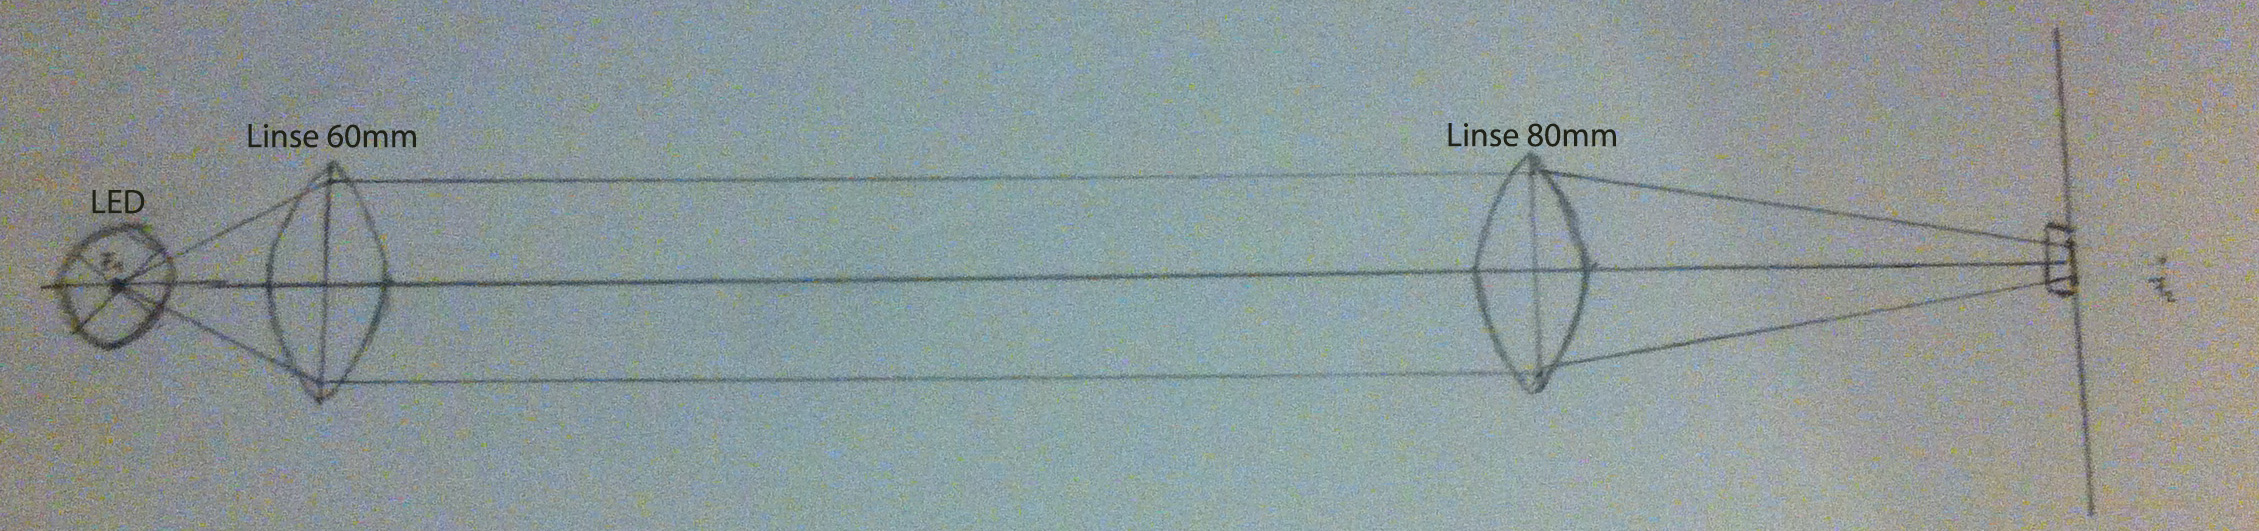
\includegraphics[width=150mm]{img/skizzen/versuch_a.jpg}
\caption{Versuchsaufbau zur Bestimmung der P-I-Kennlinie der LED}
\label{PI-Kennlinie-LED}
\end{figure}

Wir erhalten folgende Messwerte:

\begin{center}
  \begin{tabular}{|p{3.5cm}|p{4cm}|p{5cm}|}
    \hline
        Strom in mA & Leistung P in W & Fehler $\Delta$P der Leistung in W \\ \hline
        0 & $-7,799 \cdot 10^{-11}$ & $-7,799 \cdot 10^{-13}$ \\ \hline
        5 & $7,875 \cdot 10^-4$ & $7,875 \cdot 10^-6$ \\ \hline
        10 & $1,453 \cdot 10^-3$ & $1,453 \cdot 10^-5$ \\ \hline
        15 & $2,011 \cdot 10^-3$ & $2,011 \cdot 10^-5$ \\ \hline
        20 & $2,478 \cdot 10^-3$ & $2,478 \cdot 10^-5$ \\ \hline
        25 & $2,883 \cdot 10^-3$ & $2,883 \cdot 10^-5$ \\ \hline
        30 & $3,218 \cdot 10^-3$ & $3,218 \cdot 10^-5$ \\ \hline
        35 & $3,505 \cdot 10^-3$ & $3,505 \cdot 10^-5$ \\ \hline
        40 & $3,748 \cdot 10^-3$ & $3,748 \cdot 10^-5$ \\ \hline
        45 & $3,958 \cdot 10^-3$ & $3,958 \cdot 10^-5$ \\ \hline
        50 & $4,136 \cdot 10^-3$ & $4,136 \cdot 10^-5$ \\ \hline
	\end{tabular}
\end{center}

Als Fehler für die Stromstärke wurden 0.05mA angenommen, da die Stromquelle nur eine Nachkommastelle anzeigte. Dagegen wurde als Fehler für die aufgenommene Leistung 1 Prozent angenommen. Zwar ist das verwendete Messgerät deutlich genauer, allerdings wurden dennoch offensichtliche Schwankungen in der gemessenen Leistung beobachtet, welche entweder durch den im Raum verwendeten Monitor oder durch eine nicht konstante Leistung der LED verursacht wurden.

\section{Auslöschungsverhältniss der Linearpolarisatoren}
Zur Bestimmung des Auslöschungsverhältnisses der Linearpolarisatoren wurden in den Aufbau aus Abschnitt~\ref{sec:pikennlinie} noch 2 Linearpolarisatoren eingefügt.
Anschließend wurde einer der Polarisatoren so lange gedreht, bis die aufgenommene Leistung ein Minimum erreicht hat, die Polarisationsachsen der Polarisatoren also um 90° zueinander verdreht waren. Danach wurde der vordere Linearpolarisator um 90° gedreht und es wurde erneut die gemessene Leistung aufgenommen.

\begin{figure}[ht!]
\centering
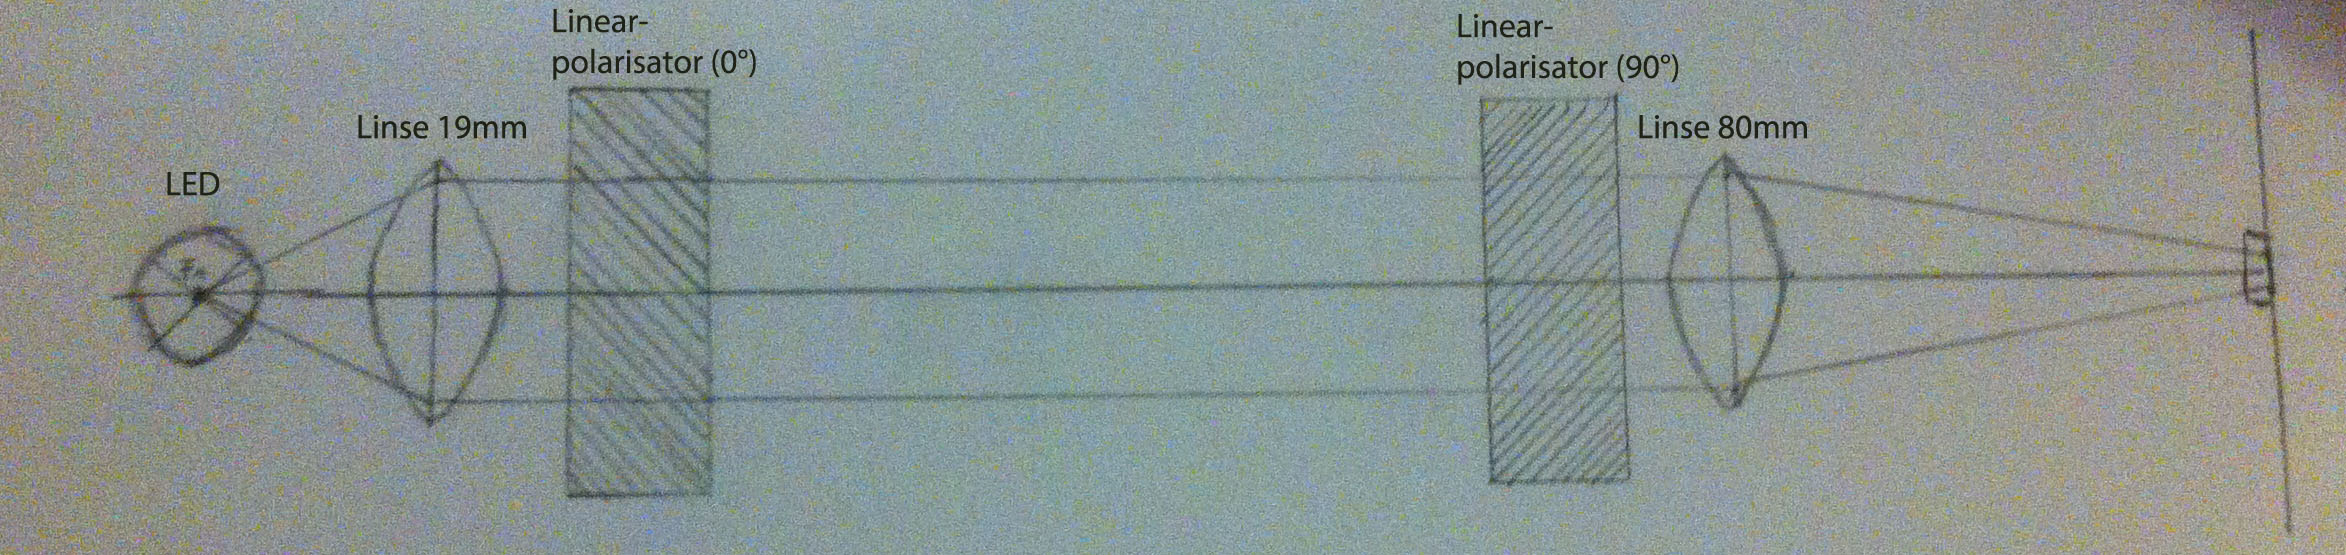
\includegraphics[width=150mm]{img/skizzen/versuch_b.jpg}
\caption{Versuchsaufbau zur Bestimmung des Auslöschungsverhältnisses der Linearpolarisatoren}
\label{Auslöschungsverhältniss-Linearpolarisatoren}
\end{figure}
Folgende Werte wurden aufgenommen:
\begin{center}
  \begin{tabular}{|p{5cm}|p{4cm}|p{4.5cm}|}
    \hline
        Winkel $\alpha$ zwischen den Polarisationsachsen in Grad & Leistung P in W & Fehler $\Delta$P der Leistung in W \\ \hline
        90 & $6,75 \cdot 10^-9$ & $0,05 \cdot 10^-9$ \\ \hline
        0 & $5,111 \cdot 10^-4$ & $0,05 \cdot 10^-4$ \\ \hline
	\end{tabular}
\end{center}
\section{Bestimmung der wellenlängenaufgelösten Verzögerung des achromatischen Verzögerungsplättchens}
Im Abschnitt 2.4 wurde bereits das $\frac{\lambda}{4}$-Plättchen beschrieben. Die schon genannte Wellenlängenabhängigkeit der tatsächlichen Phasenverschiebung soll nun untersucht werden. Zu diesem Zweck verwendenden wir den Babinet-Soleil-Kompensator. 

\begin{figure}[ht!]
\centering
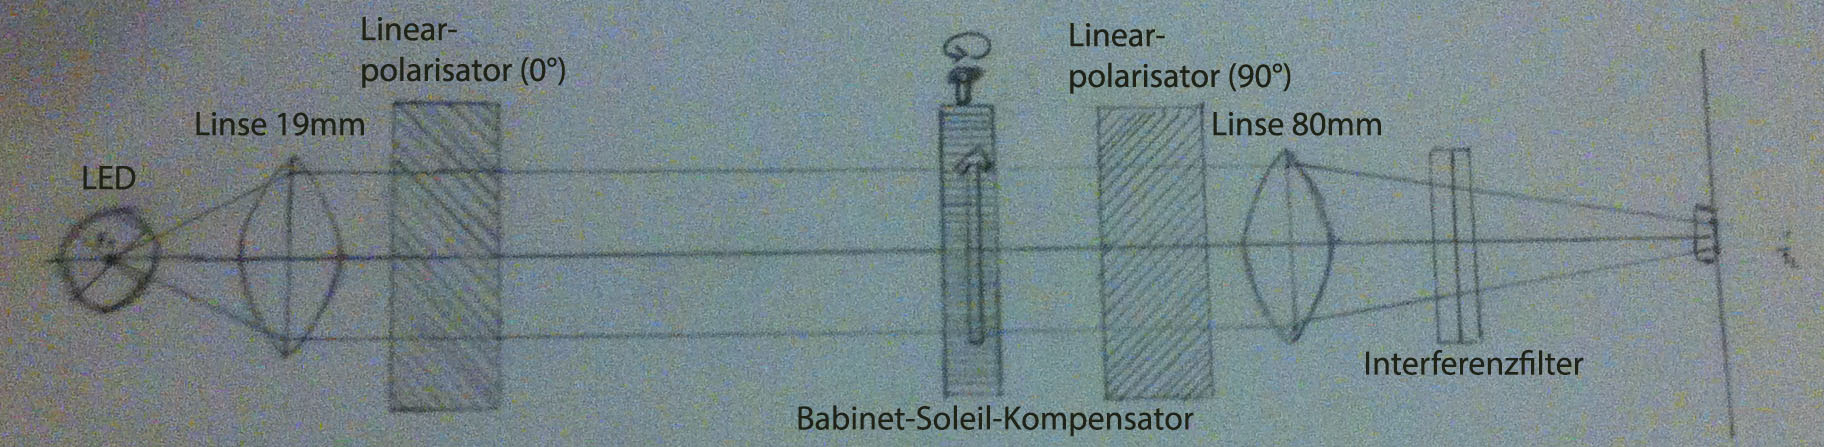
\includegraphics[width=150mm]{img/skizzen/versuch_c_1.jpg}
\caption{Versuchsaufbau zur Kalibration des BSK}
\end{figure}

Da Leistungsminima am einfachsten gemessen werden können, fügen wir den BSK  zwischen beide Polarisatoren ein, die wir vorher senkrecht zueinander ausgerichtet haben (immer in Bezug auf die optischen Achsen) und richten ihn so aus, dass immernoch ein Minimum gemessen wird. Nun verdrehen wir ihn um 45 Grad und justieren die Dicke solange nach, bis drei nebeneinanderliegende Minima gemessen werden können. Diese Minima entstehen dadurch, dass der Babinet-Soleil-Kompensator die Phasen der senkrecht aufeinander stehenden Strahlkomponenten um ganzzahlige Wellenlängen zueinander verschiebt. Diese Messungen führen wir mit verschiedenen Farbfiltern durch, jeweils bei 488 nm, 543,5 nm, 633 nm und 694,3 nm, um eine Referenz zu finden.

Bei den verwendeten Farbfiltern handelt es sich um Interferenzfilter, das heißt sie bestehen aus vielen Schichten, die sich in Brechungsindex und Dicke unterscheiden. Das einfallende Licht wird in den jeweiligen Schichten teilweise reflektiert und transmittiert und durch konstruktive und destruktive Interferenz wird erreicht, dass insgesamt lediglich ein schmaler Wellenlängenbereich transmittiert wird. Folgende Werte lesen wir am BSK ab, wobei wir den Fehler mit 0,06 abschätzen: 


\begin{center}
  \begin{tabular}{|c|c|c|c|}
    \hline
        Filter 1 (488 nm) & Filter 2 (543,5 nm) & Filter 3 (633 nm) & Filter 4 (694,3 nm) \\ \hline
        30,91 & 29,47 & 27,11 & 25,64 \\ \hline
        42,19 & 42,21 & 42,22 & 42,24 \\ \hline
        53,55 & 54,95 & 57,29 & 58,80 \\ \hline
	\end{tabular}
\end{center}

Aus den Differenzen jeweils zweier Messwerte und anschließender Mittelwertbildung können die Kalibrierungsfaktoren mit einem Fehler von etwa 0,04 ($\frac{0,06}{\sqrt{2}}$) bestimmt werden.

\begin{figure}[h]
  \begin{center}
    \begin{tabular}{|c|c|}
      \hline
      Wellenlänge des verwendeten Filters & Kalibrierungsfaktor \\ \hline
      488,0 nm                            & 11,32               \\ \hline
      543,5 nm                            & 12,74               \\ \hline
      633,0 nm                            & 15,09               \\ \hline
      694,3 nm                            & 16,58               \\ \hline
    \end{tabular}
  \end{center}
  \caption{Kalibrierungsfaktoren in $\frac{Einheiten}{2\pi}$für den Babinet-Soleil-Kompensator}
\end{figure}


Anschließend wird das $\frac{\lambda}{4}$-Plättchen in den Strahlengang vor den BSK integriert, nach dem Minimum ausgerichtet, um 45 Grad gedreht und die Messung wiederholt. Bei dieser Messung kommen die Minima dadurch zustande, dass der Babinet-Soleil-Kompensator den Einfluss der Lambda-viertel Platte gerade wieder neutralisiert.

\begin{figure}[h]
  \centering
    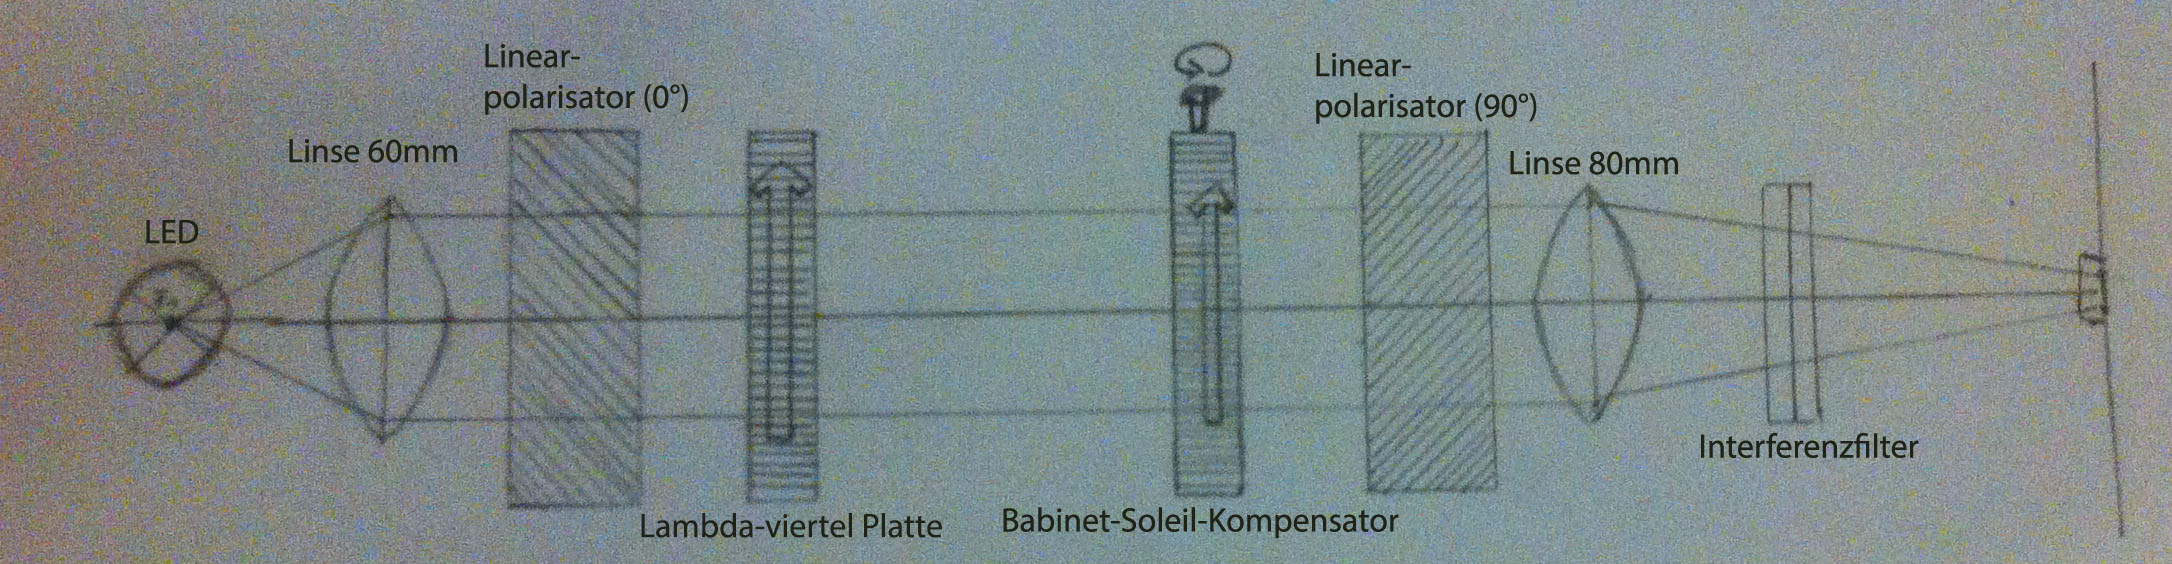
\includegraphics[width=150mm]{img/skizzen/versuch_c_2.jpg}
    \caption{Versuchsaufbau zur Bestimmung der genauen Verzögerung des Verzögerungsplättchens}
\end{figure}

Dies liefert uns folgende Werte:

\begin{center}
  \begin{tabular}{|c|c|c|c|}
    \hline
        Filter 1 (488nm) & Filter 2 (543,5nm) & Filter 3 (633nm) & Filter 4 (694,3nm) \\ \hline
        27,97 & 26,18 & 23,41 & 21,60 \\ \hline
        39,33 & 38,95 & 38,48 & 38,22 \\ \hline
        50,62 & 51,67 & 53,50 & 54,81 \\ \hline
	\end{tabular}
\end{center}

Zieht man nun die zuvor ermittelten Werte von denen mit $\frac{\lambda}{4}$-Plättchen ab, erhält man einen durch das Plättchen verursachten Offset in den von dem Babinet-Soleil-Kompensator abgelesenen Einheiten. Teilt man nun durch die zuvor bestimmten Kalibrierungsfaktoren, ergibt sich die durch das $\frac{\lambda}{4}$-Plättchen verursachte Phasenverschiebung. Anschließend kann zur Reduktion des Fehlers über die 3 errechneten Werte gemittelt werden.

An Hand dieser gemittelten Werte ergibt sich für die Phasenverzögerung der verwendeten Verzögerungsplatte:

\begin{center}
  \begin{tabular}{|c|c|}
    \hline
        Wellenlänge des verwendeten Filters & Phasenverzögerung im $\frac{\lambda}{4}$-Plättchen \\ \hline
        488,0 m                              & $(0,5177 \pm 0,0073)\pi$                           \\ \hline
        543,5 nm                              & $(0,5149 \pm 0,0065)\pi$                           \\ \hline
        633,0 nm                              & $(0,4957 \pm 0,0055)\pi$                           \\ \hline
        694,3 nm                              & $(0,4849 \pm 0,0050)\pi$                           \\ \hline
  \end{tabular}
\end{center}
\FloatBarrier


\section{Charakterisierung des Polarisationszustandes mit Hilfe des Stokes-Formalismus}
Zur Herstellung linearer Polarisation stehen uns die bekannten Glan-Thomson-Polarisationsprismen zur Verfügung. Um daraus zirkular polarisiertes Licht zu erzeugen, bedienen wir uns des $\frac{\lambda}{4}$-Plättchens, dessen Verzögerung wir im vorigen Abschnitt für die jeweiligen Wellenlängen genau bestimmt haben. Im Folgenden werden alle Messungen mit Filter 4 (694,3 nm) durchgeführt. Zunächst messen wir ohne $\frac{\lambda}{4}$-Plättchen, richten den ersten Linearpolarisator in y-Richtung aus und nehmen die Leistung über der Winkelposition des Drehwinkelaufnehmers mit $\frac{\lambda}{4}$-Plättchen auf (wir verwenden also lediglich den Drehwinkelaufnehmer mit Verzögerungsplatte, der restliche Aufbau bleibt unangetastet).

\begin{figure}[ht!]
\centering
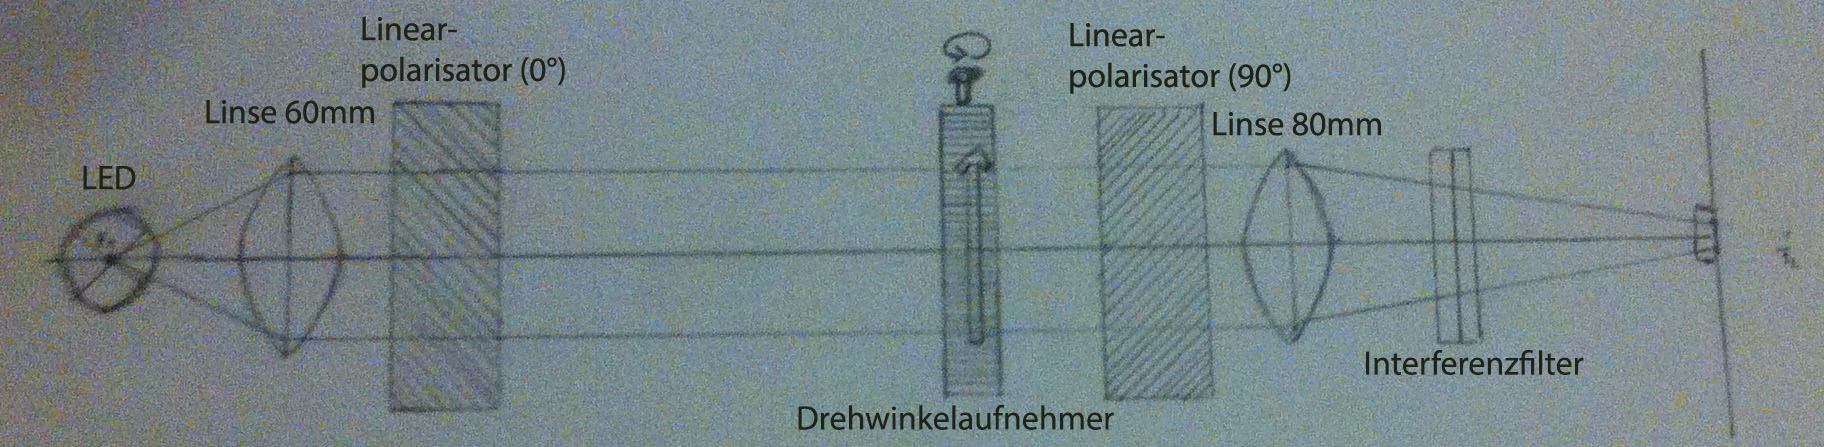
\includegraphics[width=150mm]{img/skizzen/versuch_34_1.jpg}
\caption{Versuchsaufbau mit in y-Richtung linear polarisiertem Licht}
\end{figure}

Wir erhalten folgende Verteilung:

\begin{center}
\begin{figure}[H]
\begin{tikzpicture}
\begin{axis}[
    legend pos=south west,
    title={Lichtleistung über dem Drehwinkel},
    xlabel=Drehwinkel in Grad,
    ylabel=Lichtleistung in W,
    width=0.9\textwidth,
    height=9cm,
    xmin=0,
    xmax=360,
    grid=both,
    ymin=0,
    ymax=0.000006,
    tick align=outside,
    tickpos=left,
    minor x tick num=3,
    minor y tick num=4,
    minor grid style={dotted,thin},
    seperators
]
\addplot[red, only marks, mark=x, mark size=1pt, error bars/.cd, y dir=both, y fixed relative = 0.01, x dir=both, x fixed = 0]
table[x index={0},y index={1}] {data/d-lin-y.txt};
\addlegendentry{In y-Richtung polarisiertes Licht}
\end{axis}
\end{tikzpicture}
\captionof{figure}{Linear in y-Richtung polarisiertes Licht}
\end{figure}
\end{center}

Anschließend wird der 1. Polarisator um 45$^\circ$ gedreht und die Lichtleistung erneut über der Winkelposition des $\frac{\lambda}{4}$-Plättchens aufgenommen.
\begin{figure}[ht!]
\centering
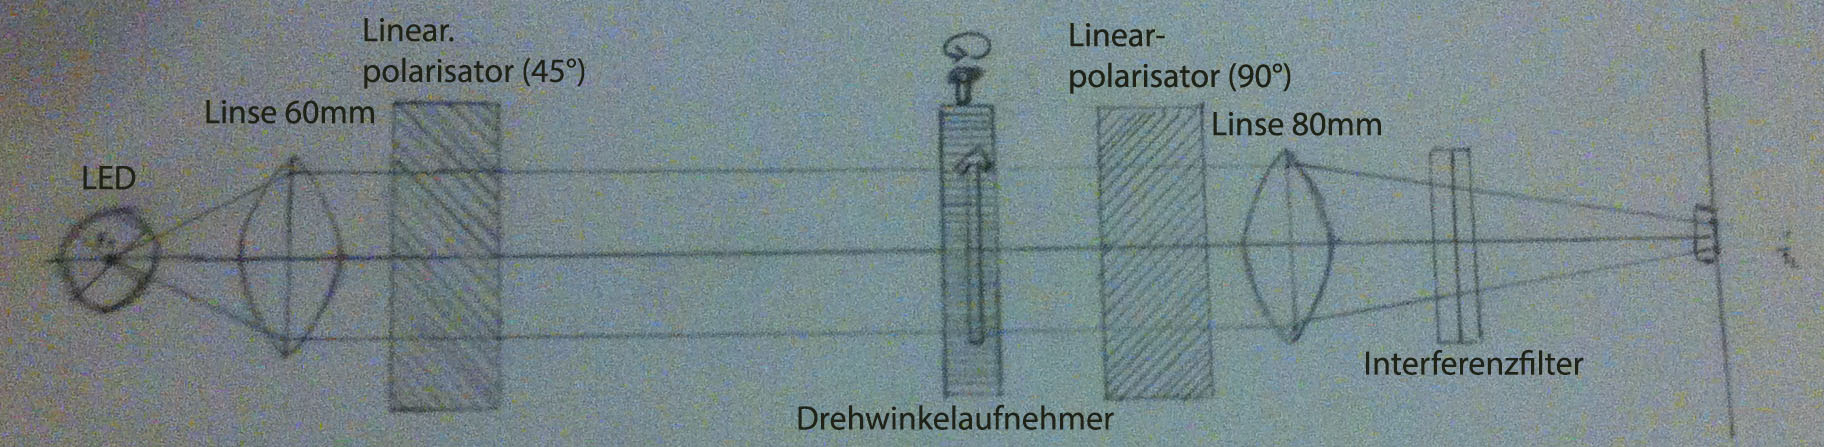
\includegraphics[width=150mm]{img/skizzen/versuch_34_2.jpg}
\caption{Versuchsaufbau mit um 45° zur y-Richtung gedrehtem, linear polarisiertem Licht}
\end{figure}

\begin{center}
\begin{figure}[H]
\begin{tikzpicture}
\begin{axis}[
    legend pos=south west,
    title={Lichtleistung über dem Drehwinkel},
    xlabel=Drehwinkel in Grad,
    ylabel=Lichtleistung in W,
    width=0.9\textwidth,
    height=9cm,
    xmin=0,
    xmax=360,
    grid=both,
    ymin=0.000002,
    ymax=0.000009,
    tick align=outside,
    tickpos=left,
    minor x tick num=3,
    minor y tick num=4,
    minor grid style={dotted,thin},
    seperators
]
\addplot[red, only marks, mark=x, mark size=1pt, error bars/.cd, y dir=both, y fixed relative = 0.01, x dir=both, x fixed = 0]
table[x index={0},y index={1}] {data/d-45.txt};
\addlegendentry{45° zur y-Richtung polarisiertes Licht}
\end{axis}
\end{tikzpicture}
\end{figure}
\end{center}

Nun untersuchen wir noch zirkular polarisiertes Licht, indem wir ein $\frac{\lambda}{4}$-Plättchen gemäß folgender Skizze hinter den vorderen Linearpolarisator einfügen. 
\begin{figure}[ht!]
\centering
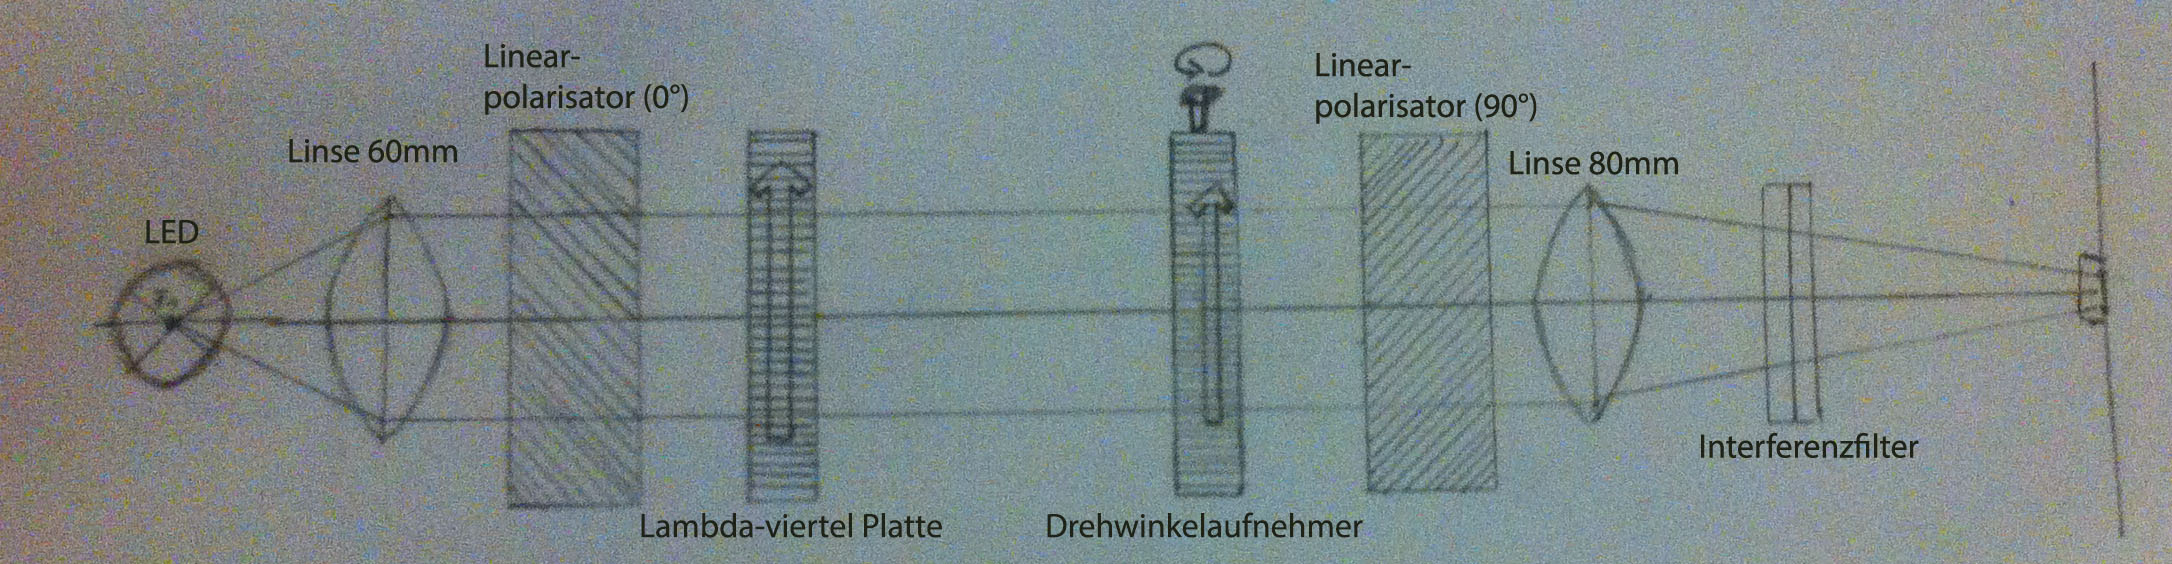
\includegraphics[width=150mm]{img/skizzen/versuch_34_3.jpg}
\caption{Versuchsaufbau mit zirkular polarisiertem Licht}
\end{figure}

Es ergeben sich folgende Messwerte:

\begin{center}
\begin{figure}[H]
\begin{tikzpicture}
\begin{axis}[
    legend pos=south west,
    title={Lichtleistung über dem Drehwinkel (Zirkular polarisiertes Licht)},
    xlabel=Drehwinkel in Grad,
    ylabel=Lichtleistung in W,
    width=0.9\textwidth,
    height=9cm,
    xmin=0,
    xmax=360,
    grid=both,
    ymin=0,
    ymax=0.000012,
    tick align=outside,
    tickpos=left,
    minor x tick num=3,
    minor y tick num=4,
    minor grid style={dotted,thin},
    seperators
]
\addplot[red, only marks, mark=x, mark size=1pt, error bars/.cd, y dir=both, y fixed relative = 0.01, x dir=both, x fixed = 0]
table[x index={0},y index={1}] {data/d-zirkular.txt};
\addlegendentry{Zirkular polarisiertes Licht}
\end{axis}
\end{tikzpicture}
%\captionof{figure}{}
\end{figure}
\end{center}


Zusätzlich steht uns eine 3D-Kinobrille zur Verfügung, deren optische Eigenschaften genauer untersucht werden sollen. Dazu montieren wir sie auf den Reiter zwischen Linse und Drehwinkelaufnehmer, zunächst so, dass das Licht der LED von innen auf das Brillenglas fällt, das Licht also in Blickrichtung des Brillenträgers propagiert. Wir messen wieder die Lichtleistung über der Winkelposition des Drehwinkelaufnehmers mit $\frac{\lambda}{4}$-Plättchen.

\begin{figure}[ht!]
\centering
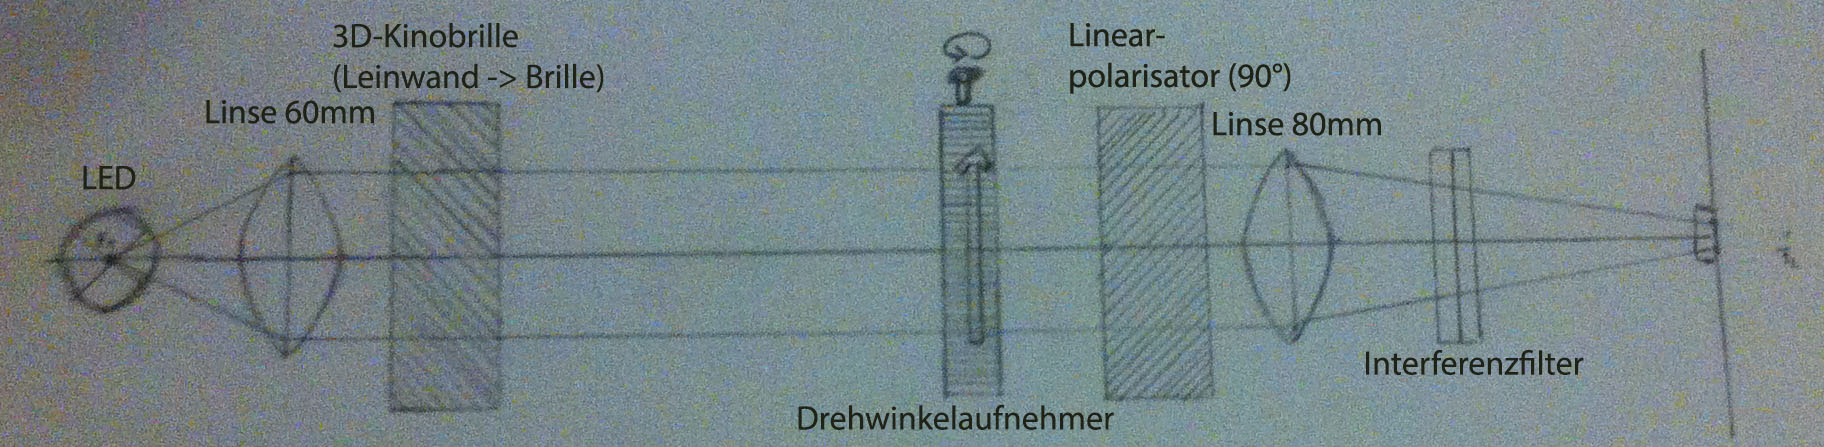
\includegraphics[width=150mm]{img/skizzen/versuch_34_4.jpg}
\caption{Versuchsaufbau mit 3D-Brille (Strahlverlauf wie von einer Leinwand zur Brille)}
\end{figure}

\begin{center}
\begin{figure}[H]
\begin{tikzpicture}
\begin{axis}[
    legend pos=south west,
    title={Lichtleistung über dem Drehwinkel},
    xlabel=Drehwinkel in Grad,
    ylabel=Lichtleistung in W,
    width=0.9\textwidth,
    height= 8cm,
    xmin=0,
    xmax=360,
    grid=both,
    ymin=0,
    ymax=0.000016,
    tick align=outside,
    tickpos=left,
    minor x tick num=3,
    minor y tick num=4,
    minor grid style={dotted,thin},
    seperators
]
\addplot[red, only marks, mark=x, mark size=1pt, error bars/.cd, y dir=both, y fixed relative = 0.01, x dir=both, x fixed = 0]
table[x index={0},y index={1}] {data/d-brille-1-licht in sichtrichtung.txt};
%\addlegendentry{}
\end{axis}
\end{tikzpicture}
\captionof{figure}{3D-Kinobrille, Lichtbestrahlung in Blickrichtung des Brillenträgers}
\end{figure}
\end{center}

Nun wiederholen wir dieselbe Messung, jedoch drehen wir die Brille um, so dass das Licht in entgegengesetzter Richtung auf das Brillenglas fällt (entgegen der Blickrichtung des Brillenträgers).
\begin{figure}[ht!]
\centering
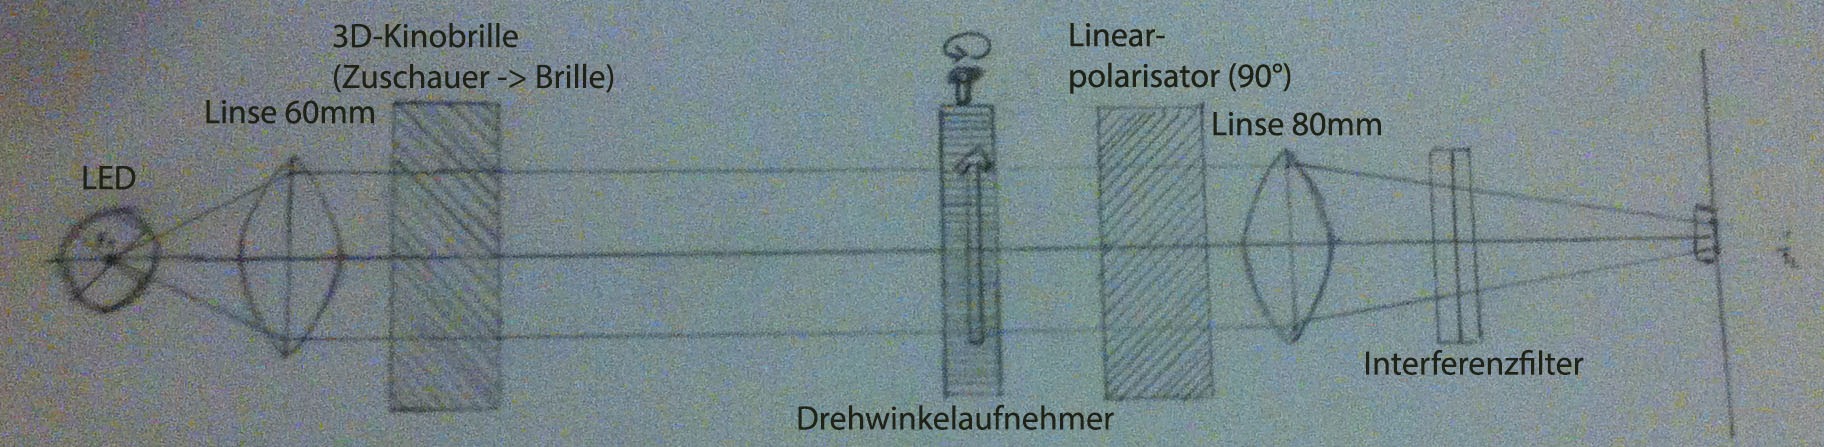
\includegraphics[width=150mm]{img/skizzen/versuch_34_5.jpg}
\caption{Versuchsaufbau mit 3D-Brille (Strahlverlauf wie von einem Zuschauer durch die Brille zur Leinwand)}
\end{figure}

\begin{center}
\begin{figure}[H]
\begin{tikzpicture}
\begin{axis}[
    legend pos=south west,
    title={Lichtleistung über dem Drehwinkel},
    xlabel=Drehwinkel in Grad,
    ylabel=Lichtleistung in W,
    width=0.9\textwidth,
    height= 8cm,
    xmin=0,
    xmax=360,
    grid=both,
    ymin=0.000007,
    ymax=0.000016,
    tick align=outside,
    tickpos=left,
    minor x tick num=3,
    minor y tick num=4,
    minor grid style={dotted,thin},
    seperators
]
\addplot[red, only marks, mark=x, mark size=1pt, error bars/.cd, y dir=both, y fixed relative = 0.01, x dir=both, x fixed = 0]
table[x index={0},y index={1}] {data/d-brille-2.txt};
%\addlegendentry{}
\end{axis}
\end{tikzpicture}
\captionof{figure}{3D-Kinobrille, Lichtbestrahlung gegen Blickrichtung des Brillenträgers}
\end{figure}
\end{center}

\section{P-I-Kennlinie der VCSEL}

Analog zur Aufnahme der P-I-Kennlinie der LED nehmen wir ebenfalls die P-I-Kennlinie des VCSELs auf. Hierzu wird im Aufbau die LED mit dem VCSEL ausgetauscht und auf die erste Linse zur Kollimation des Lichts verzichtet, da der VCSEL bereits kollimiertes Licht emittiert.

\begin{figure}[ht!]
\centering
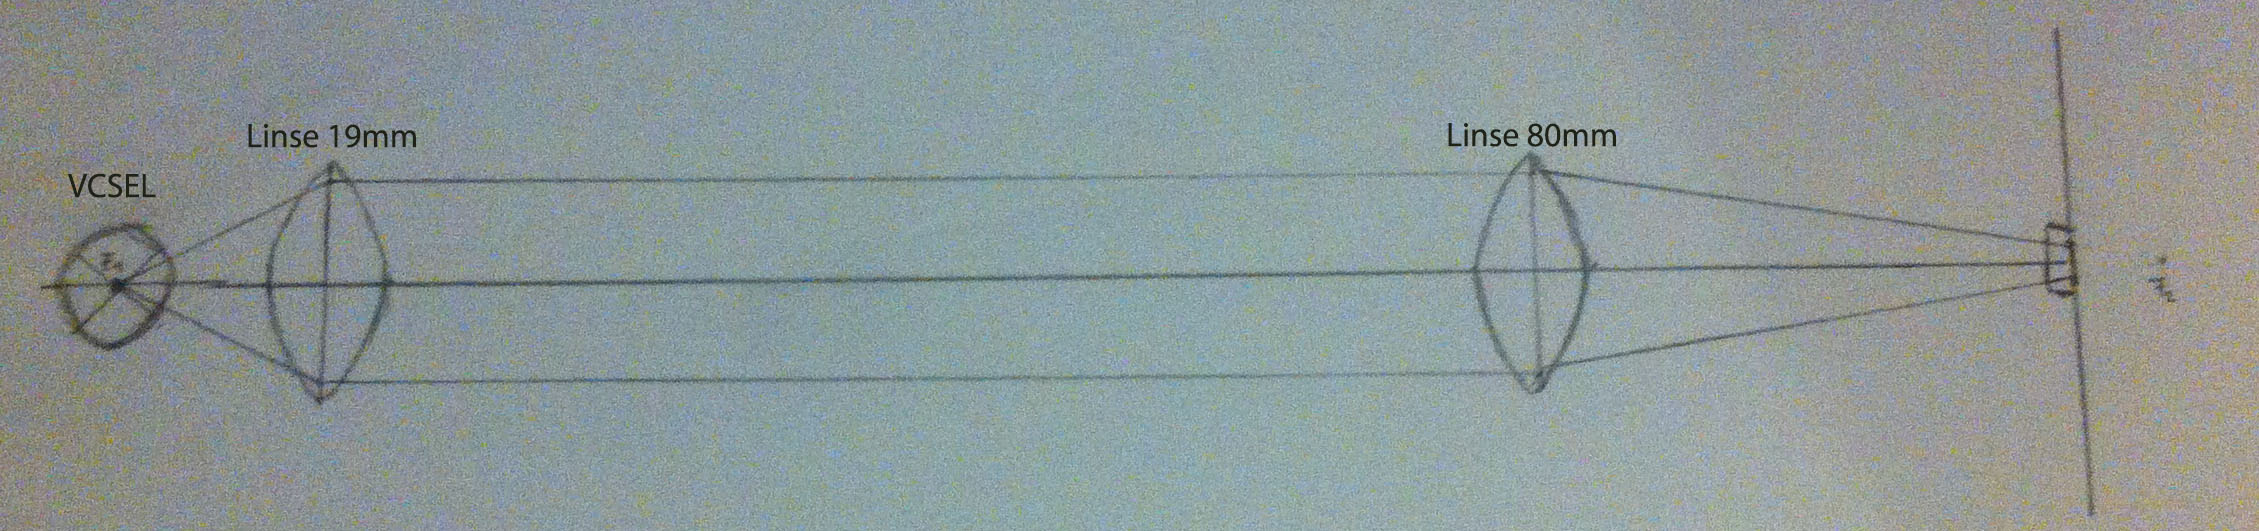
\includegraphics[width=150mm]{img/skizzen/versuch_35.jpg}
\caption{Versuchsaufbau zur Bestimmung der P-I-Kennlinie der VCSEL}
\end{figure}

Analog zu Abschnitt 3.1 wurde als Fehler für die Stromstärke 0.05mA und als Fehler für die aufgenommene Leistung 1 Prozent angenommen.

\section{Polarisationszustand des VCSELs in Abhägigkeit des Stroms}
VCSEL haben in der Regel keine feste Polarisation, vielmehr variiert die Art und der Grad der Polarisation aufgrund von thermischer Ausdehnung einzelner Komponenten mit der angelegten Stromstärke. Zur Untersuchung dieser Eigenschaft haben wir die winkelabhängige Leistung des VCSELs mit Hilfe des Drehwinkelaufnehmers bei 1 mA, 2 mA, 2,5 mA, 3 mA, 3,5 mA, 4 mA, 6 mA, 8 mA, 10 mA und 12 mA bestimmt.

Dazu wurde der vom VCSEL emittierte Strahl zuerst durch einen Linearpolarisator, dann durch den Drehwinkelaufnehmer und anschließend durch einen um 90° verdrehten Linearpolarisator gelenkt.

\begin{figure}[h]
\begin{tikzpicture}
\begin{polaraxis}[
  PolarStyle,
  ymin=-9e-7,
  ymax=9e-7,
  name=first
]
\addplot[red, only marks, mark=x, mark size=2pt]
table[x index=0,y index=1] {data/f-1.txt};
\addlegendentry{1mA}
\end{polaraxis}

\begin{polaraxis}[
  PolarStyle,
  name=second,
  at=(first.outer south east),
  anchor=outer south west
]
\addplot[blue, only marks, mark=x, mark size=2pt]
table[x index=0,y index=1, data cs=polar] {data/f-2.txt};
\addlegendentry{2mA}
\end{polaraxis}

\begin{polaraxis}[
  PolarStyle,
  name=third,
  at=(first.outer south west),
  anchor=outer north west,
  yshift=-0.25cm
]
\addplot[orange, only marks, mark=x, mark size=2pt]
table[x index=0,y index=1, data cs=polar] {data/f-2,5.txt};
\addlegendentry{2,5mA}
\end{polaraxis}

\begin{polaraxis}[
  PolarStyle,
  name=fourth,
  at=(third.outer south east),
  anchor=outer south west
]
\addplot[black, only marks, mark=x, mark size=2pt]
table[x index=0,y index=1, data cs=polar] {data/f-3.txt};
\addlegendentry{3mA}
\end{polaraxis}
\end{tikzpicture}
\captionof{figure}{Leistung in Abhängigkeit der Ausrichtung des Drehwinkelmessers für einen angelegten Strom von 1 mA, 2 mA, 2,5 mA und 3 mA. Es ist eindeutig eine Zunahme des Polarisationsgrades des emittierten Lichtes zu sehen. Bei 3mA ist bereits eine deutliche Polarisation feststellbar}
\end{figure}

\begin{figure}[h]
\begin{tikzpicture}
\begin{polaraxis}[
  PolarStyle,
  name=first
]
\addplot[red, only marks, mark=x, mark size=2pt]
table[x index=0,y index=1, data cs=polar] {data/f-3,5.txt};
\addlegendentry{3.5mA}
\end{polaraxis}

\begin{polaraxis}[
  PolarStyle,
  name=second,
  at=(first.outer south east),
  anchor=outer south west
]
\addplot[blue, only marks, mark=x, mark size=2pt]
table[x index=0,y index=1, data cs=polar] {data/f-4.txt};
\addlegendentry{4mA}
\end{polaraxis}

\begin{polaraxis}[
  PolarStyle,
  name=third,
  at=(first.outer south west),
  anchor=outer north west,
  yshift=-0.25cm
]
\addplot[orange, only marks, mark=x, mark size=2pt]
table[x index=0,y index=1, data cs=polar] {data/f-6.txt};
\addlegendentry{6mA}
\end{polaraxis}

\begin{polaraxis}[
  PolarStyle,
  name=fourth,
  at=(third.outer south east),
  anchor=outer south west
]
\addplot[black, only marks, mark=x, mark size=2pt]
table[x index=0,y index=1, data cs=polar] {data/f-8.txt};
\addlegendentry{8mA}
\end{polaraxis}

\begin{polaraxis}[
  PolarStyle,
  name=fith,
  at=(third.outer south west),
  anchor=outer north west,
  yshift=-0.25cm
]
\addplot[brown, only marks, mark=x, mark size=2pt]
table[x index=0,y index=1, data cs=polar] {data/f-10.txt};
\addlegendentry{10mA}
\end{polaraxis}

\begin{polaraxis}[
  PolarStyle,
  name=sixth,
  at=(fith.outer south east),
  anchor=outer south west
]
\addplot[purple, only marks, mark=x, mark size=2pt]
table[x index=0,y index=1, data cs=polar] {data/f-12.txt};
\addlegendentry{12mA}
\end{polaraxis}
\end{tikzpicture}
\captionof{figure}{Leistung in Abhängigkeit der Ausrichtung des Drehwinkelmessers für einen angelegten Strom von 3,5 mA, 4 mA, 6 mA, 8 mA, 10 mA und 12 mA. Die Polarisation wird durchgehend stärker und ist linear.}
\end{figure}

\chapter{Auswertung}
\section{Aufnahme der P-I-Kennlinie der LED}

Die unter Abschnitt 3.2 aufgelisteten Messwerte ergeben linear aufgetragen folgende Kennlinie:

\begin{center}
\begin{figure}[h]
\begin{tikzpicture}
\begin{axis}[
    legend pos=south west,
    title={Leistung der weißen LED in Abhängigkeit der Stromstärke},
    xlabel=Stromstärke in mA,
    ylabel=Leistung in W,
    width=0.9\textwidth,
    height= 9cm,
    xmin=0,
    xmax=55,
    grid=both,
    ymin=0,
    ymax=0.0045,
    tick align=outside,
    tickpos=left,
    minor x tick num=3,
    minor y tick num=4,
    minor grid style={dotted,thin},
    seperators
]
\addplot[red, only marks, mark=x, mark size=1pt, error bars/.cd, y dir=both, y fixed relative=0.01, x dir=both, x fixed=0.05]
table[x index={0},y index={1}] {data/1.txt};
\addlegendentry{Leistung der VCSEL auf der Photoplatte}
\end{axis}
\end{tikzpicture}
\captionof{figure}{Gemessene Leistung der VCSEL auf der Photoplatte in Abhängigkeit von der angelegten Stromstärke. Die angenommenen Fehler für die Stromstärke und die gemessene Leistung der LED betragen 0.05 mA und 1 Prozent.}
\end{figure}
\end{center}

Bis etwa 20 mA nimmt die Lichtleistung der LED angenähert proportional zur angelegten Stromstärke zu, danach steigt die Leistung nur noch langsam. Dies entspricht auch den Erwartungen, da die annähernd proportionale Zunahme der Lichtleistung nur bei konstanter Halbleitertemperatur gilt, sich aber die Temperatur ab einer gewissen elektrischen Leistung erhöht. Der Wirkungsgrad der LED sinkt folglich mit zunehmender Temperatur, wodurch die Lichtausbeute in Relation zur Leistungsaufnahme je nach Kühlung mehr oder weniger stark abnimmt. Werden LEDs nicht ausreichend gekühlt beziehungsweise mit einem dauerhaft zu hohem Strom betrieben, altern sie vorzeitig bis hin zum Totalausfall (wenn die Halbleitertemperatur 150 $^{\circ}$C längere Zeit übersteigt).

\section{Auslöschungsverhältnis der Linearpolarisatoren}
Aus den für die beiden Linearpolarisatoren aufgenommenen Werten
\begin{center}
  \begin{tabular}{|p{5cm}|p{4cm}|p{4.5cm}|}
    \hline
        Winkel $\alpha$ zwischen den Polarisationsachsen in Grad & Leistung P in W & Fehler $\Delta$P der Leistung in W \\ \hline
        90 & $6,75 \cdot 10^{-9}$ & $0,05 \cdot 10^{-9}$ \\ \hline
        0 & $5,111 \cdot 10^{-4}$ & $0,05 \cdot 10^{-4}$ \\ \hline
	\end{tabular}
\end{center}

lässt sich das Auslöschungsverhätlnis inklusive Fehler mit
\begin{align*}
  \frac{P_{min}}{P_{max}} &= \frac{6,75*10^{-9} W}{5,111*10^{-4} W} = 1,321*10^{-5} \\
  \Delta\frac{P_{min}}{P_{max}} &= \sqrt{\left(\frac{\Delta P_{min}}{P_{max}}\right)^2 + \left(\Delta P_{max} \cdot \frac{P_{min}}{P_{max}^2}\right)^2} = 1,62 * 10^{-7}
\end{align*}

berechnen. Somit ist das Auslöschungsverhältnis
\begin{align*}
\frac{P_{min}}{P_{max}} =\left(1,321\pm0,016\right) \cdot 10^{-5}
\end{align*}
\section{Bestimmung der wellenlängenaufgelösten Verzögerung des achromatischen Verzögerungsplättchens}

Aus den gemessenen Daten ergeben sich nach Mittelung folgende Verteilung für die genaue Verzögerung des Verzögerungsplättchens:
\begin{center}
  \begin{tabular}{|c|c|c|}
    \hline
        Wellenlänge des einfallenden Lichts in nm & Kalibrierungsfaktor & Phasenverschiebung in Grad \\ \hline
        $488,0 \pm 6$                             & $11,32 \pm 0,04$              & $93,18 \pm 1,31$           \\ \hline
        $543,5 \pm 6$                             & $12,74 \pm 0,04$              & $92,68 \pm 1,17$           \\ \hline
        $633,0 \pm 6$                             & $15,09 \pm 0,04$              & $89,22 \pm 0,98$           \\ \hline
        $694,3 \pm 6$                             & $16,58 \pm 0,04$              & $87,28 \pm 0,89$           \\ \hline
	\end{tabular}
\end{center}

Die Lage der Messwerte suggeriert eine lineare Abhängigkeit der Phasenverschiebung zur Wellenlänge. In der folgenden Graphik sind die Messwerte mit Fit- und Fehlergeraden zu sehen

\begin{center}
\begin{figure}[h]
\begin{tikzpicture}
\begin{axis}[
    legend pos=south east,
    title={Phasenverschiebung in Abhängigkeit der Wellenlänge},
    xlabel=Wellenlänge in nm,
    ylabel=Phasenverschiebung in Grad,
    width=0.9\textwidth,
    height= 9cm,
    xmin=450,
    xmax=730,
    grid=both,
    ymin=85,
    ymax=95,
    tick align=outside,
    tickpos=left,
    minor x tick num=3,
    minor y tick num=4,
    minor grid style={dotted,thin},
    seperators
]
\addplot[red, only marks, mark=x, mark size=1pt, error bars/.cd, y dir=both, y explicit, x dir=both, x fixed=6.00]
table[x index={0}, y index={1}, y error index={2}] {data/delta.txt};
\addlegendentry{Gemittelte Messwerte}
\end{axis}
\end{tikzpicture}
\captionof{figure}{Wellenlängenabhängige Phasenverschiebung des Verzögerungsplättchens. Der Fehler der Wellenlänge kann mit 6 nm angenommen werden, da die Halbwertsbreite $10 \pm 2$ beträgt (Quelle: Datenblatt), den Fehler der abgelesenen Werte m BSK haben wir mit 0,06 abgeschätzt.}
\end{figure}
\end{center}
\FloatBarrier

\section{Charakterisierung des Polarisationszustandes mit Hilfe des Stokes-Formalismus}

Aus den gewonnenen Verteilungen der Lichtleistung über dem Drehwinkel sollen nun die Stokes-Parameter berechnet werden, um die Polarisation klassifizieren zu können. Wir bedienen uns dazu des Müller-Matrix-Formalismus, wir multiplizieren also die Müller-Matrizen der verwendeten optischen Bauteile. Dies sind im Wesentlichen ein Verzögerungsplättchen, welches beim verwendeten Filter 4 (694,3 nm) eine Phasenverschiebung von $115,08^\circ \pm 0,99^\circ$ verursacht und mit der x-Achse den Winkel $\beta$ einschließt (Der Winkel $\beta$ ist derjenige, der per Drehwinkelaufnehmer variiert wurde) und ein Glan-Thomson-Polarisator, der mit der x-Achse den Winkel $\alpha = 0$ einschließt. Die Multiplikation liefert die Intensität in Abhängigkeit des Winkels $\beta$ für eine Phasenverschiebung von $\delta=\frac{\pi}{2}$: 

$$I_T(\beta) = \frac{1}{2} (S_0 + cos(2 \beta) (S_1 cos(2 \beta) + S_2 sin(2 \beta)) - sin(2 \beta) \cdot S_3 )$$

Es fällt auf, dass es sich um eine $2 \pi$-periodische Funktion handelt, das heißt wir können die Intensität als Fourierreihe darstellen: 

$$I_T(\beta) = \frac{1}{2} [S_0 + \frac{1}{2} S_1 - S_3 sin(2 \beta) + \frac{1}{2} S_1 cos(4 \beta) + \frac{1}{2} S_2 sin(4 \beta)]$$

Mit den Fourierkoeffizienten $C0, C2, C4, S2, S4$ ergibt sich: 

$$I_T(\beta) = C0 + C2 \cdot cos(2 \beta) + S2 \cdot sin (2 \beta) + C4 \cdot cos (4 \beta) + S4 \cdot sin (4 \beta)$$

Dies bietet sich auch vor allem deshalb an, weil man nun die Darstellung diskretisieren kann, um die (ebenfalls diskreten) Messwerte zur Berechnung der Fourierkoeffizienten verwenden zu können:

\begin{align*}
 C0 &= \frac{1}{N} \sum_{i=1}^N I_{Ti},\\
 C2 &= \frac{2}{N} \sum_{i=1}^N I_{Ti} cos(2 \beta_i),\\
 C4 &= \frac{2}{N} \sum_{i=1}^N I_{Ti} cos(4 \beta_i),\\
 S2 &= \frac{2}{N} \sum_{i=1}^N I_{Ti} sin(2 \beta_i),\\
 S4 &= \frac{2}{N} \sum_{i=1}^N I_{Ti} sin(4 \beta_i)
\end{align*}

Der Index i repräsentiert den i-ten Messwert jeweils der Intensität und des Winkels, das heißt wir summieren in 72 Schritten die Messwerte auf und erhalten damit für jede der 4 Messaufbauten einen Satz von Fourierkoeffizienten.

Aus den Fourierkoeffizienten lassen sich nun die gesuchten Stokes-Parameter wie folgt berechnen, wobei bereits die Werte für $\alpha$ und $\beta_0$ eingesetzt wurden: 

\begin{align*}
 S_0 &= C0 - C4 \frac{1 + cos(\delta)}{1 - cos(\delta)},\\ 
 S_1 &= C4 \frac{2}{1 - cos(\delta)},\\
 S_2 &= S4 \frac{2}{1 - cos(\delta)},\\
 S_3 &= \frac{-S2}{sin(\delta)} 
\end{align*}

Wir können also die erzeugten Polarisationszustände mit 5 Sätzen von Stokes-Parametern klassifizieren. Die oben beschriebene Rechnung führen wir mit Mathematica durch und erhalten für jede Messung die normierten Stokes-Parameter:

\begin{figure}[h]
  \begin{center}
    \begin{tabular}{|p{3.6cm}|p{0.9cm}|p{2.7cm}|p{2.7cm}|p{2.7cm}|p{2.3cm}|}
      \hline
      Polarisationsfilter        & $S_0$   & $S_1$              & $S_2$              & $S_3$               & DOP               \\ \hline
      Linearpolarisator 0°       & $1,00 $ & $-0,996 \pm 0,019$ & $0,142 \pm 0,078$  & $0,0023 \pm 0,0000$ & $1,006 \pm 0,029$ \\ \hline
      Linearpolarisator 45°      & $1,00 $ & $-0,115 \pm 0,072$ & $0,926 \pm 0,018$  & $0,0015 \pm 0,0000$ & $0,934 \pm 0,049$ \\ \hline
      $\frac{\lambda}{4}$-Platte & $1,00 $ & $-0,065 \pm 0,002$ & $0,026 \pm 0,005$  & $0,9877 \pm 0,0007$ & $0,990 \pm 0,002$ \\ \hline
      3D-Brille 1                & $1,00 $ & $0,465 \pm 0,009$  & $0,063 \pm 0,036$  & $0,8837 \pm 0,0006$ & $1,000 \pm 0,010$ \\ \hline
      3D-Brille 2                & $1,00 $ & $1,027 \pm 0,017$  & $-0,018 \pm 0,080$ & $0,0029 \pm 0,0000$ & $1,027 \pm 0,024$ \\ \hline
    \end{tabular}
  \end{center}
  \caption{Normierte Stokes-Parameter.Die 3D-Brille wurde zuerst so angebracht, dass das Licht den gleichen weg wie in einem Kino nimmt. Anschließend wurde dir 3D-Brille um 180° Gedreht, so dass das Einfallende Licht zuerst den Benutzer-zugewandten Teil der Brille pasiert}
\end{figure}

Die genauen Messaufbauten sind unter 3.4 näher beschrieben.

Als Fehler für $\alpha$ und $\beta_0$ haben wir jeweils 1 Grad angenommen, der Fehler für $\delta$ wurde aus Abschnitt 4.3 übernommen.

Damit erschließt sich auch die Funktionsweise der 3D-Brille:
Sie ist (in Blickrichtung) aus einem Linearpolarisator gefolgt von einer Verzögerungsplatte aufgebaut. Das von der Leinwand kommende, links- und rechtszirkular polarisierte Licht wird so zuerst in 2 um 90 Grad gedrehte linear polarisierte Anteile aufgespalten und überlagert sich anschließend wieder im Auge. Die beiden unterschiedlich zirkular polarisierten Anteile stellen verschiedene Bildebenen dar, die leicht zueinander verschoben sind, wodurch der 3-D-Eindruck entsteht.

\section{P-I-Kennlinie der VCSEL}
Bis zu einer angelegten Stromstärke von etwa 3 mA steigt die Leistung des VCSELs nur sehr langsam an. Dies kann dadurch erklärt werden, dass im Vergleich zu Absorption im VCSEL die Verstärkung im Resonator nur gering ist, also kaum oder keine Verstärkung stattfindet. Die anschließende annähernd linear ansteigende Leistung verhält sich wie in einem typischen Laserresonator, wobei im Gegensatz zu makroskopischen Resonatoren der Anstieg der Leistung mit zunehmender Stromstärke wieder abnimmt. Dies ist dadurch zu erklären, dass aufgrund der geringen Länge der einzelnen Resonatorschichten bereits kleine Längenänderungen im Resonator die Verstärkung beeinträchtigen kann.

\begin{center}
\begin{figure}[h]
\begin{tikzpicture}
\begin{axis}[
    legend pos=south east,
    title={Leistung der VCSEL in Abhängigkeit der Stromstärke},
    xlabel=Stromstärke in mA,
    ylabel=Leistung in W,
    width=0.9\textwidth,
    height= 9cm,
    xmin=0,
    xmax=13,
    grid=both,
    ymin=0,
    ymax=0.0022,
    tick align=outside,
    tickpos=left,
    minor x tick num=3,
    minor y tick num=4,
    minor grid style={dotted,thin},
    seperators
]
\addplot[red, only marks, mark=x, mark size=1pt, error bars/.cd, y dir=both, y fixed relative=0.01, x dir=both, x fixed=0.05]
table[x index={0},y index={1}] {data/e-P-I.txt};
\addlegendentry{Leistung der VCSEL auf der Photoplatte}
\end{axis}
\end{tikzpicture}
\captionof{figure}{Gemessene Leistung der VCSEL auf der Photoplatte in Abhängigkeit von der angelegten Stromstärke. Die angenommenen Fehler für die Stromstärke und die gemessene Leistung der VCSEL betragen 0.05mA und 1 Prozent.}
\end{figure}
\end{center}

Im Bezug auf den Laserschutz macht die aufgenommene Leistung von wenigen Milliwatt das Tragen von Schutzbrillen erforderlich, besondere Vorsichtsmaßnahmen, um nicht mit dem Strahl in Kontakt zu kommen, müssen jedoch nicht getroffen werden.

\section{Polarisationszustand des VCSELs in Abhängigkeit des Stroms}
Mit Hilfe des bereits in Abschnitt 4.4 beschriebenen Verfahrens lässt sich aus den winkelabhängigen Intensitäten der Stokes-Vektor und somit der Grad der Polarisation des vom VCSEL emittierten Lichtes bestimmen. Stromstärkenabhängig ergeben sich die folgenden Werte für den normierten Stokes-Vektor und den Grad der Polarisation:

\begin{center}
  \begin{tabular}{|c|c|c|c|c|c|}
    \hline
        Strom in mA & $S_{0}$ & $S_{1}$ & $S_{2}$ & $S_{3}$ & Polarisationsgrad \\ \hline
        $1,0 \pm 0,05 $ & $1$ & $-0,0317 \pm 0,0016$ & $0,0165 \pm 0,0025$ & $-0,0006 \pm 0,0000$ & $0,0357 \pm 0,0017$ \\ \hline
        $2,0 \pm 0,05 $ & $1$ & $-0,0646 \pm 0,0027$ & $0,0304 \pm 0,0051$ & $-0,0020 \pm 0,0000$ & $0,0714 \pm 0,0032$ \\ \hline
        $2,5 \pm 0,05 $ & $1$ & $-0,1410 \pm 0,0041$ & $0,0610 \pm 0,0111$ & $-0,0033 \pm 0,0000$ & $0,1537 \pm 0,0067$ \\ \hline
        $3,0 \pm 0,05 $ & $1$ & $-0,7020 \pm 0,0261$ & $0,2908 \pm 0,0551$ & $-0,0077 \pm 0,0000$ & $0,7599 \pm 0,0354$ \\ \hline
        $3,5 \pm 0,05 $ & $1$ & $-0,8045 \pm 0,0302$ & $0,3362 \pm 0,0631$ & $-0,0049 \pm 0,0000$ & $0,8720 \pm 0,0420$ \\ \hline
        $4,0 \pm 0,05 $ & $1$ & $-0,8283 \pm 0,0318$ & $0,3571 \pm 0,0650$ & $-0,0043 \pm 0,0000$ & $0,9020 \pm 0,0445$ \\ \hline
        $6,0 \pm 0,05 $ & $1$ & $-0,8377 \pm 0,8373$ & $0,3628 \pm 0,0323$ & $-0,0019 \pm 0,0000$ & $0,9125 \pm 0,0452$ \\ \hline
        $8,0 \pm 0,05 $ & $1$ & $-0,7115 \pm 0,0373$ & $0,6792 \pm 0,0546$ & $-0,0028 \pm 0,0000$ & $0,9837 \pm 0,0667$ \\ \hline
        $10,0\pm 0,05 $ & $1$ & $-0,8127 \pm 0,0320$ & $0,3625 \pm 0,0638$ & $-0,0048 \pm 0,0000$ & $0,8899 \pm 0,0445$ \\ \hline
        $12,0\pm 0,05 $ & $1$ & $-0,7794 \pm 0,0315$ & $0,3590 \pm 0,0612$ & $-0,0055 \pm 0,0000$ & $0,8582 \pm 0,0433$ \\ \hline
	\end{tabular}
\end{center}

Auch hier haben wir als Fehler für $\alpha$ und $\beta_0$ jeweils 1 Grad angenommen, der Fehler für $\delta$ war vorgegeben. Grafisch veranschaulicht sind die Stokes-Parameter in folgenden Diagrammen:

\begin{center}
\begin{figure}[H]
\begin{tikzpicture}
\begin{axis}[
    legend pos=south east,
    title={$S_1$ in Abhängigkeit der Stromstärke},
    xlabel=Stromstärke in mA,
    ylabel=$S_1$,
    width=0.9\textwidth,
    height=8.5cm,
    xmin=0,
    xmax=13,
    grid=both,
    ymin=-1,
    ymax=0,
    tick align=outside,
    tickpos=left,
    minor x tick num=3,
    minor y tick num=4,
    minor grid style={dotted,thin},
    seperators
]
\addplot[red, only marks, mark=x, mark size=1pt, error bars/.cd, y dir=both, y fixed relative=0.04, x dir=both, x fixed=0.05]
table[x index={0},y index={1}] {data/S1.txt};
%\addlegendentry{Stokes-Parameter $S_1$ in Abhängigkeit des Stroms}
\end{axis}
\end{tikzpicture}
\captionof{figure}{Berechneter Wert $S_1$ in Abhängigkeit der angelegten Stromstärke. Die angenommenen Fehler für $\alpha$ und $\beta_0$ betragen je 1$^{\circ}$, der für den Strom beträgt 0,05 mA}
\end{figure}
\end{center}

\begin{center}
\begin{figure}[H]
\begin{tikzpicture}
\begin{axis}[
    legend pos=south east,
    title={$S_2$ in Abhängigkeit der Stromstärke},
    xlabel=Stromstärke in mA,
    ylabel=$S_2$,
    width=0.9\textwidth,
    height=8.5cm,
    xmin=0,
    xmax=13,
    grid=both,
    ymin=0,
    ymax=0.7,
    tick align=outside,
    tickpos=left,
    minor x tick num=3,
    minor y tick num=4,
    minor grid style={dotted,thin},
    seperators
]
\addplot[red, only marks, mark=x, mark size=1pt, error bars/.cd, y dir=both, y fixed relative=0.04, x dir=both, x fixed=0.05]
table[x index={0},y index={1}] {data/S2.txt};
%\addlegendentry{Stokes-Parameter $S_2$ in Abhängigkeit des Stroms}
\end{axis}
\end{tikzpicture}
\captionof{figure}{Berechneter Wert $S_2$ in Abhängigkeit der angelegten Stromstärke. Die angenommenen Fehler für $\alpha$ und $\beta_0$ betragen je 1$^{\circ}$, der für den Strom beträgt 0,05 mA}
\end{figure}
\end{center}

\begin{center}
\begin{figure}[H]
\begin{tikzpicture}
\begin{axis}[
    legend pos=south east,
    title={$S_3$ in Abhängigkeit der Stromstärke},
    xlabel=Stromstärke in mA,
    ylabel=$S_3$,
    width=0.9\textwidth,
    height=8.5cm,
    xmin=0,
    xmax=13,
    grid=both,
    ymin=-0.01,
    ymax=0,
    tick align=outside,
    tickpos=left,
    minor x tick num=3,
    minor y tick num=4,
    minor grid style={dotted,thin},
    seperators
]
\addplot[red, only marks, mark=x, mark size=1pt, error bars/.cd, y dir=both, y fixed relative=0, x dir=both, x fixed=0.05]
table[x index={0},y index={1}] {data/S3.txt};
%\addlegendentry{Stokes-Parameter $S_3$ in Abhängigkeit des Stroms}
\end{axis}
\end{tikzpicture}
\captionof{figure}{Berechneter Wert $S_3$ in Abhängigkeit der angelegten Stromstärke. Die angenommenen Fehler für $\alpha$ und $\beta_0$ betragen je 1$^{\circ}$, der für den Strom beträgt 0,05 mA}
\end{figure}
\end{center}

Der Polarisationsgrad lässt sich ebenfalls anhand einer Grafik sofort ablesen: 

\begin{center}
\begin{figure}[H]
\begin{tikzpicture}
\begin{axis}[
    legend pos=south east,
    title={Grad der Polarisation in Abhängigkeit von der Stromstärke},
    xlabel=Stromstärke in mA,
    ylabel=Grad der Polarisation,
    width=0.9\textwidth,
    height= 8cm,
    xmin=0,
    xmax=13,
    grid=both,
    ymin=0,
    ymax=1.15,
    tick align=outside,
    tickpos=left,
    minor x tick num=3,
    minor y tick num=4,
    minor grid style={dotted,thin},
    seperators,
    seperators
]
\addplot[red, only marks, mark=x, mark size=1pt, error bars/.cd, y dir=both, y explicit, x dir=both, x explicit]
table[x index={0}, x error index={1}, y index={2}, y error index={3}] {data/f-stokes.txt};
%\addlegendentry{Leistung der LED auf der Photoplatte}
\end{axis}
\end{tikzpicture}
\captionof{figure}{Polarisationsgrad in Abhängigkeit der Stromstärke}
\end{figure}
\end{center}
\FloatBarrier 

Offensichtlich steigt der Grad der Polarisation zu Beginn stark an und erreicht dann von 4 mA bis etwa 10 mA ein Plateau mit einem Maximum bei 8 mA. Dies lässt sich durch thermische Ausdehnung im Laserresonator erklären. Offensichtlich scheint die Temperatur, welche in der Nähe von 8 mA im VCSEL vorliegt, ideal für eine Polarisation des Lichts zu sein. Da die thermische Ausdehnung bei steigender Stromstärke noch weiter steigt, nimmt die Polarisation bei höheren Stromstärken wieder ab.

Die gemessenen Werte zeigen eine eindeutige lineare Polarisation des emittierten Lichts, der zirkular polarisierte Anteil ist durchweg vernachlässigbar.

\chapter{Fazit}
In diesem Versuch gelang es uns, verschiedene Polarisationsarten mit Hilfe des Stokes-Formalismus zu untersuchen. So wurden in Abschnitt 4.4 sowohl linear polarisiertes Licht in y-Richtung als auch zirkular polarisiertes Licht untersucht. Ebenfalls linear polarisiertes Licht und die Abhängigkeit des Polarisationsgrads eines VCSELs von der angelegten Stromstärke wurde in Abschnitt 4.6 genauer untersucht. Auffällig dabei war, dass bei einer angelegten Stromstärke von 8 mA beinahe vollständige Polarisation des emittierten Lichts erreicht wurde.

Auch haben wir den Aufbau einer 3D-Brille untersucht und herausgefunden, dass sie (in Blickrichtung gesehen) aus einem Linearpolarisator gefolgt von einer Verzögerungsplatte aufgebaut ist.

Grundsätzlich ist zunächst festzustellen, dass die Berechnung der Stokes-Parameter beziehungsweise der Stokes-Vektoren aus den Messdaten gut gelungen ist, insbesondere da die Untersuchung des präparierten Lichts sich mit den Erwartungen sehr gut gedeckt hat. Z.B. bei der Ausrichtung des Linearpolarisators nach der y-Achse konnte die entsprechende lineare Polarisation auch sehr gut durch den Stokes-Vektor nachgewiesen werden. Bei der Herstellung von zirkular polarisiertem Licht ist die Abweichung (der entsprechende Stokes-Parameter beträgt 0,987 statt 1) immer noch klein, jedoch etwas größer, was sich wohl durch die Abweichung der Phasenverschiebung, die durch das Verzögerungsplättchen verursacht wird, erklären lässt. Das heißt um ganz genau zu sein, hätte das Verzögerungsplättchen in einem Winkel montiert werden müssen, der von 45$^{\circ}$ geringfügig abweicht. Durch die begrenzte zur Verfügung stehende Zeit müssen hier Abstriche gemacht werden; der Grundstein für das Verständnis der Wellenlängenabhängigkeit der Phasenverschiebung wurde aber gelegt, indem diese separat untersucht wurde. 

Weiterhin vermittelt der Versuch ein Gefühl für den Umgang und die Messmethoden mit optischen Komponenten, z.B. war zu beachten, dass keine Fehlmessungen durch Lichtreflexionen oder Fremdstrahlungsquellen ausgelöst wurden. Eine leichte Verfälschung ließ sich nicht ganz vermeiden, da selbst im abgedunkelten Raum z.B. das Licht des verwendeten Computermonitors durch Reflexionen an heller Kleidung o.ä. oder durch einen ungünstigen Winkel des Monitors zur Messapparatur Einfluss haben kann. Durch Beachtung dieser Punkte konnte das Risiko für Fehlmessungen minimiert werden, was letztlich auch verwertbare und verlässliche Messdaten liefert.

Es ist auch klar geworden, wie man Polarisation von Licht messen kann. Der Detektor misst nämlich lediglich die Lichtleistung, das heißt etwa durch Verdrehen würde sich keine Änderung einstellen. Man muss immer mit Polarisatoren arbeiten, um Aussagen über die Polarisation treffen zu können, beispielsweise kann ein Linearpolarisator rotiert werden und verändert so die gemessene Leistung in Abhängigkeit seines Winkels, wodurch dann Rückschlüsse auf die Polarisation möglich werden. Insgesamt konnte erfolgreich eine Messmethodik entwickelt und angewendet werden sowie die physikalischen Hintergründe erarbeitet werden, die zur Auswertung der Polarisationsanalyse notwendig sind.
%ENDE INHALT
\cleardoublepage{}
% Eintrag fürs Inhaltsverzeichnis
\newpage
\begin{thebibliography}{100}
  \bibitem{GefahrenLaser} \url{http://de.wikipedia.org/w/index.php?title=Laser&oldid=128632514#Gefahren}
\end{thebibliography}

\cleardoublepage{}
% Eintrag fürs Inhaltsverzeichnis
% Abbildungsverzeichnis einfügen
\end{document}
